\documentclass[a4paper]{article}

\usepackage{mathtools} % математические формулы
\usepackage[T1,T2A]{fontenc} % кириллица
\usepackage[utf8]{inputenc} % кодировка шрифта кириллицы
\usepackage{indentfirst} %делать отступ в начале параграфа
\usepackage{enumerate} % нумерация списков
\usepackage{tabularx} % таблицы
\usepackage[english,russian]{babel} % вставка стороннего текста
\usepackage[12pt]{extsizes}
\usepackage{amsthm, amssymb, amsmath, amsfonts, nccmath, empheq}
\usepackage{color,colortbl} 
\usepackage[warn]{mathtext}
\usepackage{tocloft}  % для отточий в оглавлении
\linespread{1.5}
\usepackage{setspace} % для пробелов между линий
\usepackage{cmap}


\onehalfspacing
\usepackage{float}
\usepackage{graphicx}
\graphicspath{{pictures/}}
\DeclareGraphicsExtensions{.pdf,.png,.jpg}
\usepackage[left=25mm,right=25mm,
    top=2cm,bottom=30mm,bindingoffset=0cm]{geometry}
\renewcommand{\cftsecleader}{\cftdotfill{\cftdotsep}}

\usepackage{hyperref} % для гиперссылки на гитхаб

\author{Тырыкин Я. А. }
\date{March 2021}


\begin{document}
\begin{titlepage}
    \begin{center}
        \mbox{\normalsize{Санкт-Петербургский Политехнический Университет имени Петра Великого}}\\
        \normalsize{Институт Прикладной Математики и Механики}\\
        \large{\textbf{Кафедра "Прикладная Математика"}}
        
        \vfill
        
        \textbf{\Large{Отчет по лабораторным работам №5-8}}\\
        \textbf{\large{по дисциплине}}\\
        \textbf{\large"Математическая Статистика"}
        
        \vfill
        \raggedleft{Выполнил студент:}\\
        \raggedleft{Тырыкин Я. А.}\\
        \raggedleft{группа 5030102/80401}\\
        \raggedleft{Проверил:}\\
        \raggedleft{к.ф.-м.н., доцент}\\
        \raggedleft{Баженов А. Н.}\\
        
        \vfill
    
    \end{center}
    
    \begin{center} 
        Санкт-Петербург \\
        2021 
    \end{center}
\end{titlepage}
\newpage

% страница с оглавлением
% \renewcommand{\contentsname}{Оглавление} % можно поменять название оглавление
\begin{center}
    \tableofcontents
\end{center}
\setcounter{page}{2}
\newpage

% страница со списком графиков
\begin{center}
    \listoffigures
\end{center}
\newpage

% страница со списком таблиц
\begin{center}
    \listoftables
\end{center}
\newpage


\section{Постановка задачи}
    \subsection{Лабораторная работа №5}
    Сгенерировать двумерные выборки размерами 20, 60, 100 для нормального двумерного распределения $N(x, y, 0, 0, 1, 1, \rho)$

    Коэффициент корреляции $\rho$ Коэффициент корреляции


    Каждая выборка генерируется 1000 раз и для неё вычисляются: среднее значение, среднее значение квадрата и дисперсия коэффициентов
корреляции Пирсона, Спирмена и квадрантного коэффициента корреляции.

    Повторить все вычисления для смеси нормальных распределений:
 
    \begin{center}
        $f(x, y) = 0.9N(x, y, 0, 0, 1, 1, 0.9) + 0.1N(x, y, 0, 0, 10, 10, -0.9)$.\\
    \end{center}
    
    Изобразить сгенерированные точки на плоскости и нарисовать эллипс
равновероятности.

 
\section{Теория}

    \subsection{Двумерное нормальное распределение}
    
        Двумерная случайная величина $(X, Y)$ называется распределённой нормально (или просто нормальной), если её плотность вероятности определена
формулой

        \begin{equation} \label{double_norm_distr}
            N(x, y, \overline{x}, \overline{y}, \sigma_x, \sigma_y, \rho) = \dfrac{1}{2 \pi \sigma_x \sigma_y \sqrt{1 - \rho^2}} \times \\
            \exp{(\dfrac{1}{2(1 - \rho^2)}[\dfrac{(x - \overline{x})^2}{\sigma^2_x} - 2 \rho \dfrac{(x - \overline{x})(y - \overline{y})}{\sigma_x \sigma_y} + \dfrac{(y - \overline{y})^2}{\sigma^2_y}])}
        \end{equation}
        
        Компоненты $X, Y$ двумерной нормальной случайной величины также распределены нормально с математическими ожиданиями $\overline{x}, \overline{y}$ и средними квадратическими отклонениями $\sigma_x, \sigma_y$ соответственно.
        
        Параметр $\rho$ называется коэффициентом корреляции.
    
    \subsection{Корреляционный момент (ковариация) и коэффициент корреляции}
    
        \textbf{Корреляционный момент}, иначе ковариация, двух случайных величин $X$ и $Y$:
        
        \begin{equation}\label{cov}
            K = cov(X, Y) = M[(X - \overline{x})(Y - \overline{y})].
        \end{equation}
        
        \textbf{Коэффициент корреляции} $\rho$ двух случайных величин $X$ и $Y$:
        
        \begin{equation}\label{cor}
            \rho = \dfrac{K}{\sigma_x \sigma_y}
        \end{equation}
    
    \subsection{Выборочные коэффициенты корреляции}
    
        \subsubsection{Выборочный коэффициент корреляции Пирсона}
            \textbf{Выборочный коэффициент корреляции Пирсона}:
            
            \begin{equation}\label{pearson}
                r = \dfrac{\dfrac{1}{n} \sum(x_i - \overline{x})(y_i - \overline{y})}{\sqrt{\dfrac{1}{n^2} \sum(x_i - \overline{x})^2 \sum(y_i - \overline{y})^2}} = \dfrac{K}{s_X s_Y}
            \end{equation}
            
            где $K, s^2_X, s^2_Y -$ выборочные ковариация и дисперсии случайных величин $X$ и $Y$.
            
        \subsubsection{Выборочный квадрантный коэффициент корреляции}
        
        \textbf{Выборочный квадрантный коэффициент корреляции}
        
        \begin{equation} \label{square_cor}
            r_Q = \dfrac{(n_1 + n_3) - (n_2 + n_4)}{n}
        \end{equation}
        
        где $n_1$, $n_2$, $n_3$ и $n_4 -$ — количества точек с координатами $(x_i, y_i)$, попавшими соответственно в $I$, $II$, $III$ и $IV$ квадранты декартовой системы с осями $x' = x - med x, y' = y - med y$ и с центром в точке с координатами $(med x, med y)$.
        
        \subsubsection{Выборочный коэффициент ранговой корреляции Спирмена}
            
            Обозначим ранги, соотвествующие значениям переменной $X$, через $u$,  а ранги, соотвествующие значениям переменной $Y - $ через $v$.
            
            \textbf{Выборочный коэффициент ранговой корреляции Спирмена:}
            
            \begin{equation} \label{sperman}
                r_S = \dfrac{\dfrac{1}{n} \sum(u_i - \overline{u})(v_i - \overline{v})}{\sqrt{\dfrac{1}{n^2} \sum(u_i - \overline{u})^2 \sum(v_i - \overline{v})^2}}
            \end{equation}
            
            где $\overline{u} = \overline{v} = \dfrac{1 + 2 + ... + n}{n} = \dfrac{n + 1}{2}$ - среднее значение рангов.
            
    \subsection{Эллипсы рассеивания}
        
        Уравнение проекции эллипса рассеивания на плоскость $xOy$:
        
        \begin{equation} \label{ellips}
            \dfrac{(x - \overline{x})^2}{\sigma^2_x} - 2 \rho \dfrac{(x - \overline{x})(y - \overline{y})}{\sigma_x \sigma_y} + \dfrac{(y - \overline{y})^2}{\sigma^2_y} = const
        \end{equation}
        
        Центр эллипса \eqref{ellips} находится в точке с координатами $(\overline{x}, \overline{y})$; оси симметрии эллипса составляют с осью $Ox$ углы, определяемые уравнением
        
        \begin{equation}\label{angles}
            \text{tg } 2 \alpha = \dfrac{2 \rho \sigma_x \sigma_y}{\sigma^2_x - \sigma^2_y}
        \end{equation}

\section{Модульная структура программы}

    Лабораторная работа выполнена с применением средств языка Python версии 3.7 в среде разработки PyCharm IDE (в частности, с применением встроенных методов библиотеки SciPy и MatPlotLib). Исходной код лабораторной работы находится по ссылке в приложении к отчёту.
    
\section{Результаты}

    \subsection{Выборочные коэффициенты корреляции}
    
        \begin{table}[H]
            \centering
            \begin{tabular}{|c|c|c|c|}
                \hline
                 $\rho = 0$ (\ref{cor}) & $r$ (\ref{pearson}) & $r_s$ (\ref{sperman}) & $r_Q$ (\ref{square_cor})  \\ \hline
                 $E(z)$ & -0.002 & -0.005 & 0.02  \\ \hline
                 $E(z^2)$ & 0.05 & 0.05 & 0.05  \\ \hline
                 $D(z)$ & 0.05 & 0.06 & 0.05  \\ \hline
                 & & & \\ \hline
                 $\rho = 0.5$ & $r$ & $r_s$ & $r_Q$  \\ \hline
                 $E(z)$ & 0.24 & 0.22 & 0.32  \\ \hline
                 $E(z^2)$ & 0.16 & 0.15 & 0.17  \\ \hline
                 $D(z)$ & -0.08 & -0.07 & 0.14  \\ \hline
                 & & & \\ \hline
                 $\rho = 0.9$ & $r$ & $r_s$ & $r_Q$  \\ \hline
                 $E(z)$ & 0.46 & 0.43 & 0.7  \\ \hline
                 $E(z^2)$ & 0.37 & 0.35 & 0.52  \\ \hline
                 $D(z)$ & -0.08 & -0.08 & 0.03  \\ \hline
                 
            \end{tabular}
            \caption{Двумерное нормальное распределение, $n$ = 20}
            \label{tab:normal_20}
        \end{table}
        
        \begin{table}[H]
            \centering
            \begin{tabular}{|c|c|c|c|}
                \hline
                 $\rho = 0$ (\ref{cor}) & $r$ (\ref{pearson}) & $r_s$ (\ref{sperman}) & $r_Q$ (\ref{square_cor})  \\ \hline
                 $E(z)$ & 0.34 & 0.32 & 0.001  \\ \hline
                 $E(z^2)$ & 0.28 & 0.27 & 0.02  \\ \hline
                 $D(z)$ & -0.05 & -0.05 & 0.02  \\ \hline
                 & & & \\ \hline
                 $\rho = 0.5$ & $r$ & $r_s$ & $r_Q$  \\ \hline
                 $E(z)$ & 0.37 & 0.35 & 0.33 \\ \hline
                 $E(z^2)$ & 0.28 & 0.26 & 0.13  \\ \hline
                 $D(z)$ & -0.09 & -0.09 & 0.02 \\ \hline
                 & & & \\ \hline
                 $\rho = 0.9$ & $r$ & $r_s$ & $r_Q$  \\ \hline
                 $E(z)$ & 0.46 & 0.44 & 0.7  \\ \hline
                 $E(z^2)$ & 0.36 & 0.34 & 0.5  \\ \hline
                 $D(z)$ & -0.09 & -0.09 & 0.009  \\ \hline
                 
            \end{tabular}
            \caption{Двумерное нормальное распределение, $n$ = 60}
            \label{tab:normal_60}
        \end{table}
        
        \begin{table}[H]
            \centering
            \begin{tabular}{|c|c|c|c|}
                \hline
                 $\rho = 0$ (\ref{cor}) & $r$ (\ref{pearson}) & $r_s$ (\ref{sperman}) & $r_Q$ (\ref{square_cor})  \\ \hline
                 $E(z)$ & 0.39 & 0.37 & 0.006  \\ \hline
                 $E(z^2)$ & 0.31 & 0.3 & 0.01  \\ \hline
                 $D(z)$ & -0.07 & -0.07 & 0.01  \\ \hline
                 & & & \\ \hline
                 $\rho = 0.5$ & $r$ & $r_s$ & $r_Q$  \\ \hline
                 $E(z)$ & 0.4 & 0.39 & 0.34 \\ \hline
                 $E(z^2)$ & 0.3 & 0.29 & 0.12  \\ \hline
                 $D(z)$ & -0.1 & -0.09 & 0.01  \\ \hline
                 & & & \\ \hline
                 $\rho = 0.9$ & $r$ & $r_s$ & $r_Q$  \\ \hline
                 $E(z)$ & 0.46 & 0.44 & 0.7  \\ \hline
                 $E(z^2)$ & 0.36 & 0.34 & 0.47  \\ \hline
                 $D(z)$ & -0.09 & -0.09 & 0.01  \\ \hline
                 
            \end{tabular}
            \caption{Двумерное нормальное распределение, $n$ = 100}
            \label{tab:normal_100}
        \end{table}
        
        \begin{table}[H]
            \centering
            \begin{tabular}{|c|c|c|c|}
                \hline
                 $\rho = 0$ (\ref{cor}) & $r$ (\ref{pearson}) & $r_s$ (\ref{sperman}) & $r_Q$ (\ref{square_cor})  \\ \hline
                 $E(z)$ & -0.5 & 0.43 & 0.51  \\ \hline
                 $E(z^2)$ & 0.5 & 0.26 & 0.3  \\ \hline
                 $D(z)$ & 0.3 & 0.06 & 0.04  \\ \hline
                 & & & \\ \hline
                 $\rho = 0.5$ & $r$ & $r_s$ & $r_Q$  \\ \hline
                 $E(z)$ & -0.65 & 0.47 & 0.56 \\ \hline
                 $E(z^2)$ & 0.49 & 0.25 & 0.32  \\ \hline
                 $D(z)$ & 0.05 & -0.03 & 0.01  \\ \hline
                 & & & \\ \hline
                 $\rho = 0.9$ & $r$ & $r_s$ & $r_Q$  \\ \hline
                 $E(z)$ & -0.69 & 0.47 & 0.56  \\ \hline
                 $E(z^2)$ & 0.51 & 0.24 & 0.323  \\ \hline
                 $D(z)$ & 0.03 & 0.02 & 0.007  \\ \hline
                 
            \end{tabular}
            \caption{Смесь нормальных распределений}
            \label{tab:mixed}
        \end{table}

    \subsection{Эллипсы рассеивания}
    
        \begin{figure}[H]
            \centering
            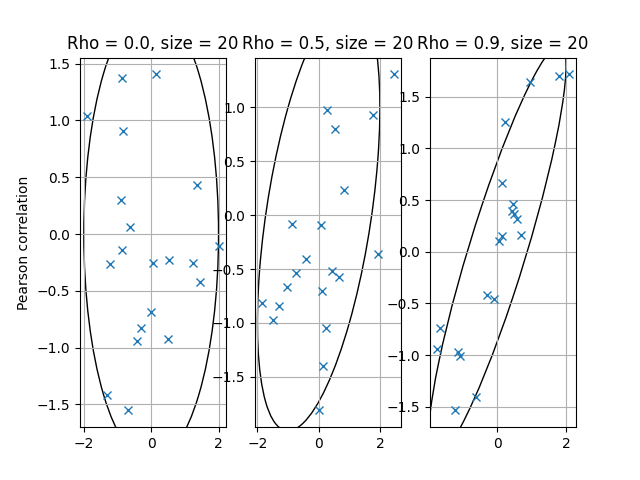
\includegraphics[scale = 0.4]{Pearson correlation, size = 20.png}
            \caption{Двумерное нормальное распределение, $n$ = 20}
            \label{fig:pearson_20}
        \end{figure}
        
        \begin{figure}[H]
            \centering
            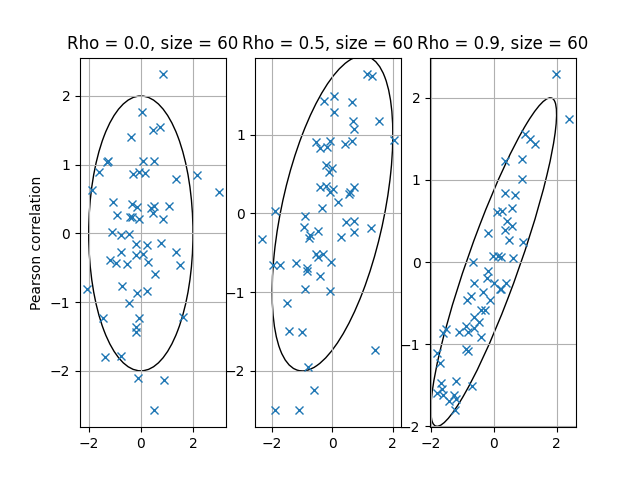
\includegraphics[scale = 0.4]{Pearson correlation, size = 60.png}
            \caption{Двумерное нормальное распределение, $n$ = 60}
            \label{fig:pearson_60}
        \end{figure}
        
         \begin{figure}[H]
            \centering
            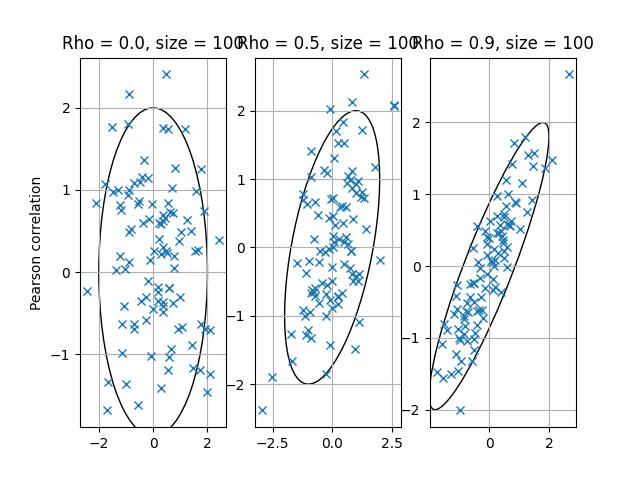
\includegraphics[scale = 0.4]{Pearson correlation, size = 100.png}
            \caption{Двумерное нормальное распределение, $n$ = 100}
            \label{fig:pearson_100}
        \end{figure}
    
\section{Обсуждение}

    \subsection{Выборочные коэффициенты корреляции и эллипсы рассеивания}
    
       Сравним дисперсии выборочных коэффициентов корреляции: \\
       
       \begin{itemize}
           \item Для двумерного нормального распределения дисперсии выборочных коэффициентов корреляции упорядочены следующим образом: $r_Q > r_s > r$.  \\
           \item Для смеси нормальных распределений дисперсии выборочных коэффициентов корреляции упорядочены следующим образом: $r_Q < r_s < r$.  \\
       \end{itemize}
        
        Процент попавших элементов выборки в эллипс рассеивания (95\%-ная доверительная область) примерно равен его теоретическому значению (95\%). \\

\section{Ресурсы}
    \begin{spacing}{2.5}
        Код программы, реализующей отрисовку обозначенных распределений:
        
        \href{https://github.com/YaroslavAggressive/Mathematical-statistics-lab-works}{https://github.com/YaroslavAggressive/Mathematical-statistics-lab-works}
    \end{spacing}
    
\end{document}
